% This is a sample document using the University of Minnesota, Morris, Computer Science
% Senior Seminar modification of the ACM sig-alternate style. Much of this content is taken
% directly from the ACM sample document illustrating the use of the sig-alternate class. Certain
% parts that we never use have been removed to simplify the example, and a few additional
% components have been added.

% See https://github.com/UMM-CSci/Senior_seminar_templates for more info and to make
% suggestions and corrections.

\documentclass{sig-alternate}
\usepackage{color}
\usepackage[colorinlistoftodos]{todonotes}

%%%%% Uncomment the following line and comment out the previous one
%%%%% to remove all comments
%%%%% NOTE: comments still occupy a line even if invisible;
%%%%% Don't write them as a separate paragraph
%\newcommand{\mycomment}[1]{}

\begin{document}

% --- Author Metadata here ---
%%% REMEMBER TO CHANGE THE SEMESTER AND YEAR AS NEEDED
\conferenceinfo{UMM CSci Senior Seminar Conference, December 2015}{Morris, MN}

\title{Heuristics for the Generalized Traveling Salesman Problem}

\numberofauthors{1}

\author{
% The command \alignauthor (no curly braces needed) should
% precede each author name, affiliation/snail-mail address and
% e-mail address. Additionally, tag each line of
% affiliation/address with \affaddr, and tag the
% e-mail address with \email.
\alignauthor
Molly Grove\\
	\affaddr{Division of Science and Mathematics}\\
	\affaddr{University of Minnesota, Morris}\\
	\affaddr{Morris, Minnesota, USA 56267}\\
	\email{grove266@morris.umn.edu}
}

\maketitle
%This color is for my comments
\definecolor{light-gray}{gray}{0.75}
\begin{abstract}
The generalized traveling salesman problem (GTSP) is a variation of the traveling salesman problem, a classic NP-hard optimization problem. The goal of the GTSP is to find a minimum-cost cycle that visits one node from every subset, or category, of vertices. This paper presents several algorithms for finding approximate solutions to the GTSP. 
\end{abstract}

\keywords{generalized traveling salesman problem, hybrid algorithms, parameterized algorithms, consultant-guided search, variable neighborhood search, combinatorial optimization}

\section{Introduction}
\label{sec:introduction}
%\todo[inline, color=light-gray]{some history of the TSP, easy vs hard problems (compare to Chinese Postman Problem?), overview of what the paper covers} 

Many problems with practical applications involve completing a required task with as little cost as possible, whether cost is defined as time, money, distance, or some other measure. While some problems, such as finding the shortest route from one location to another, are relatively easy to solve, others do not have known easy solutions. One example of this is the traveling salesman problem. The traveling salesman problem is a well-known problem where a salesman must travel to all of a specific selection of cities in one trip and wishes to find the shortest route available without repeating any cities. This problem has many applications, including some such as task scheduling where no actual traveling is involved. 

The \textit{generalized} traveling salesman problem is like the traveling salesman problem except that instead of going to every city, the cities are divided into groups and the traveler must go to one city in each group. The `cities' in each group may be relatively close together, as would be the case for a traveler going to one city in each of several states, or they may not be, as would be the case for someone running errands who needs to go to one of each of several types of stores. This means that the generalized traveling salesman problem has potential for even more variation than the traveling salesman problem. 

Like the traveling salesman problem, the generalized traveling salesman problem has many applications, and cannot be solved optimally without essentially trying all possibilities. For this reason, approximate algorithms, which give a solution that is good, but not always optimal, are used. 

This paper presents some approximate algorithms, or \textit{heuristics}, for the generalized traveling salesman problem. Section~\ref{sec:background} provides some background necessary to understand the algorithms. Section~\ref{sec:parameterized} introduces a parameterized algorithm used for road networks. Section~\ref{sec:genetic} describes a hybrid algorithm that combines several search techniques. Section~\ref{sec:VNS} introduces some search algorithms that can be combined with variable-neighborhood search, as well as some instances that illustrate why combining them is beneficial. 

%In Section~\ref{sec:VNS}, I introduce several algorithms and a method of combining them called Variable-Neighborhood Search. I then show several instances that illustrate the strengths and weaknesses of the two separate algorithms, including one instance that is hard for both of them, but where the combined algorithm results in a good approximation. 

\section{Background}
\label{sec:background}
To understand the problem and heuristics, we must first understand some graph theory, some computation theory, and the precise definition of the generalized traveling salesman problem. 

\subsection{Graphs}
\label{subs:graphs}
\begin{figure}
\centering
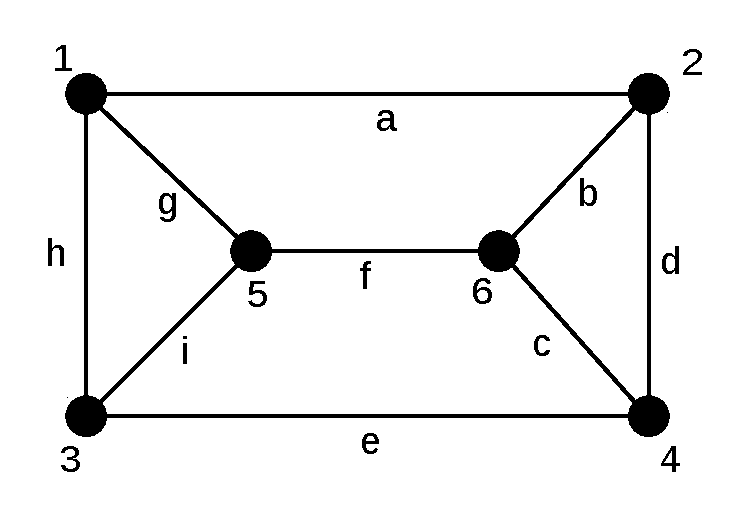
\psfig{file=graphExample.pdf,width=2in}
\caption{A graph with vertices and edges labeled}
\label{fig:graph}
\end{figure}
This section defines some graph theory terms necessary to understand the generalized traveling salesman problem. 

A \textit{graph} $G=(V,E)$ is an ordered pair of two sets: a set $V$ of \textit{vertices} and a set $E$ of \textit{edges}. Each edge is defined by a pair of vertices. For example, an edge $(a,b)$ connects vertices $a$ and $b$. The edges may have weight or cost values, $c_{i,j}$, where $(i,j)$ is an edge in $E$. Vertices are said to be \textit{adjacent} if they are connected by an edge. Vertices are sometimes referred to as \textit{nodes}, and I will be using these terms interchangeably. Figure~\ref{fig:graph} is an example of a graph with vertices and edges indicated by numbers and letters, respectively. 

In non-technical terms, a graph is a set of points (vertices or nodes) with lines (edges) connecting them. Cost values can be thought of as the cost of traversing the edges. For some applications, this corresponds to the length of the edge. 

Given a graph $G=(V,E)$, a \textit{path} is a sequence of unique nodes and edges $(v_{1}, e_{1}, v_{2}, e_{2}, ..., e_{n-1}, v_{n})$ where each node is adjacent to the previous one and the edges between the nodes connect the two nodes. For example, in Figure~\ref{fig:graph}, $(4,e,3,i,5,g,1)$ is a path. Notice that there are no repeated nodes. A \textit{cycle} is a path except that $v_{1} = v_{n}$; that is, a path that starts and ends at the same place. One example of a cycle in Figure~\ref{fig:graph} is $(2,a,1,g,5,f,6,b,2)$. Notice that the sequence has no repeated nodes except the first one, which is repeated at the end of the sequence. 

%\subsection{Computational Complexity}
%\label{subs:complexity}

%Some problems, such as the shortest path problem, are relatively easy for computers to solve optimally. For these problems, exact algorithms are often used to find the optimal solution. However, other problems do not have a known algorithm that can solve them without basically trying every possible solution. Although this may not be a problem if the number of possible solutions is small, the number of solutions is often large enough that it is not feasible to find an optimal solution. The traveling salesman problem is one of these problems. For this reason, people often use approximate algorithms for the traveling salesman problem. These algorithms don't always lead to the optimal solution. However, some of them can generate solutions that are good enough for practical purposes in a reasonable amount of time. 

\subsection{The class NP-hard}
\label{subs:NPhard}
In this section, I define some terms used to classify problems based on computational complexity. 

A \textit{decision problem} is a problem that, when solved, results in a `yes' or `no' answer \cite{Sipser:2013}. A decision problem is said to be in the class \textit{P} if, in the worst case, it can be solved by an algorithm in polynomial time \cite{Papadimitriou:1982}. A problem can be solved in \textit{polynomial time} if an algorithm with an input of size $n$ can solve the problem in no more than $n^{k}$ steps, where $k$ is a constant that does not depend on $n$. 

Exact algorithms are generally used for problems in the class P, because most computers can use polynomial time algorithms to solve them quickly enough for most practical purposes, even when $n$ is fairly large. However, there are many problems for which no polynomial-time solution has been found. 

%\begin{figure}
%\centering
%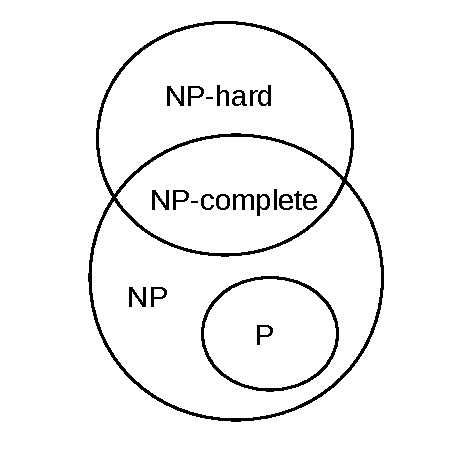
\psfig{file=NPdiagram2.pdf,width=2in}
%\caption{The classes P, NP, NP-hard, and NP-complete}
%\label{fig:NPdiagram}
%\end{figure}

A decision problem is in the class \textit{NP} if a polynomial-time algorithm can \textit{verify} it, meaning that the algorithm can check in polynomial time if a given candidate for a solution is indeed a solution. Note that this definition does not exclude problems in P. In fact, P is a subset of NP. 

There are some problems that can be proven to be at least as hard as every problem in NP. These are referred to as \textit{NP-hard}. A problem is NP-hard if every problem in NP can be \textit{polynomially reduced} to it  \cite{Papadimitriou:1982}. This means that if there is a polynomial-time algorithm that can solve an NP-hard problem, the algorithm can be changed into an algorithm to solve any problem in NP in polynomial time. 

%Problems that are in both NP and NP-hard are called NP-complete. Figure~\ref{fig:NPdiagram} shows the relationship between P, NP, NP-complete, and NP-hard. 

Because the traveling salesman problem is not a decision problem, it is not in NP. However, it is NP-hard, along with the generalized traveling salesman problem and many other optimization problems. Problems that are not in P, including NP-hard problems, are much more computationally intensive when the input is large, since the number of steps increases more quickly (often exponentially) as the input size increases. For this reason, approximate algorithms are often used for NP-hard optimization problems. These algorithms don't always lead to the optimal solution. However, some of them can generate solutions that are good enough for practical purposes in a reasonable amount of time. 

\subsection{Generalized Traveling Salesman Problem}
\label{subs:GTSP}
The generalized traveling salesman problem is, as the name suggests, a generalization of a different problem, the traveling salesman problem. 

The traveling salesman problem (TSP) is defined as follows: Given a graph $G=(V,E)$, find the minimum-cost cycle that contains all nodes in $G$. The TSP is known to be NP-hard \cite{Papadimitriou:1982}. 

In the generalized traveling salesman problem (GTSP), instead of going to all nodes, the nodes are divided into disjoint subsets and the cycle has to go to one node in each subset. Mathematically, it can be defined as follows: 
Given a graph $G=(V,E)$ and disjoint subsets $V_{1}, V_{2},...,V_{n}$ of the set $V$, find the minimum cost cycle containing one node from each subset $V_{i}$. 

Rice and Tsotras \cite{Rice:2013} show that the TSP can be reduced to the GTSP, so the GTSP is also NP-hard. 
\subsection{The Generalized Traveling Salesman Path Problem}
\label{subs:GTSPP}
The generalized traveling salesman \textit{path} problem (GTSPP) is similar to the generalized traveling salesman problem, except that the starting and ending node are defined, and they are not necessarily the same node. Formally, it can be defined as follows: Given a graph $G=(V,E)$, disjoint subsets $V_{1}, V_{2},...,V_{n}$ of the set $V$, and nodes $s$ and $t$ in $V$, find the minimum cost path from $s$ to $t$ containing one node from each subset $V_{i}$. 

Rice and Tsotras \cite{Rice:2013} show that the GTSP can be reduced to the GTSPP. Any GTSPP algorithm can also be used for the GTSP, by setting $s=t$ and taking the minimum cost over all possible choices of $s$. Since the GTSP is NP-hard, this means that the GTSPP is also NP-hard. 

\section{Parameterized Algorithms and the GTSPP}
\label{sec:parameterized}

One method of finding an approximate solution to the GTSPP or the GTSP is to use parameterized algorithms. Parameterized complexity theory defines complexity not just by the size of the input, but also by other parameters. This helps distinguish between algorithms that are inefficient in theory and practice and algorithms that are inefficient in theory but actually not that inefficient for many practical purposes. 

This section summarizes the algorithm presented by Rice and Tsotras \cite{Rice:2013}. The algorithm that follows is most useful in cases where the nodes in each node subset are scattered. This algorithm is for the GTSPP, from Section~\ref{subs:GTSPP}. However, as mentioned before, the same algorithm could be used for the GTSP. This algorithm also allows repeated nodes. 

%Additionally, this algorithm modifies the problem such that not every node is in one of the node subsets, and the path may visit more than one node in a node subset. 

\begin{figure}
\centering
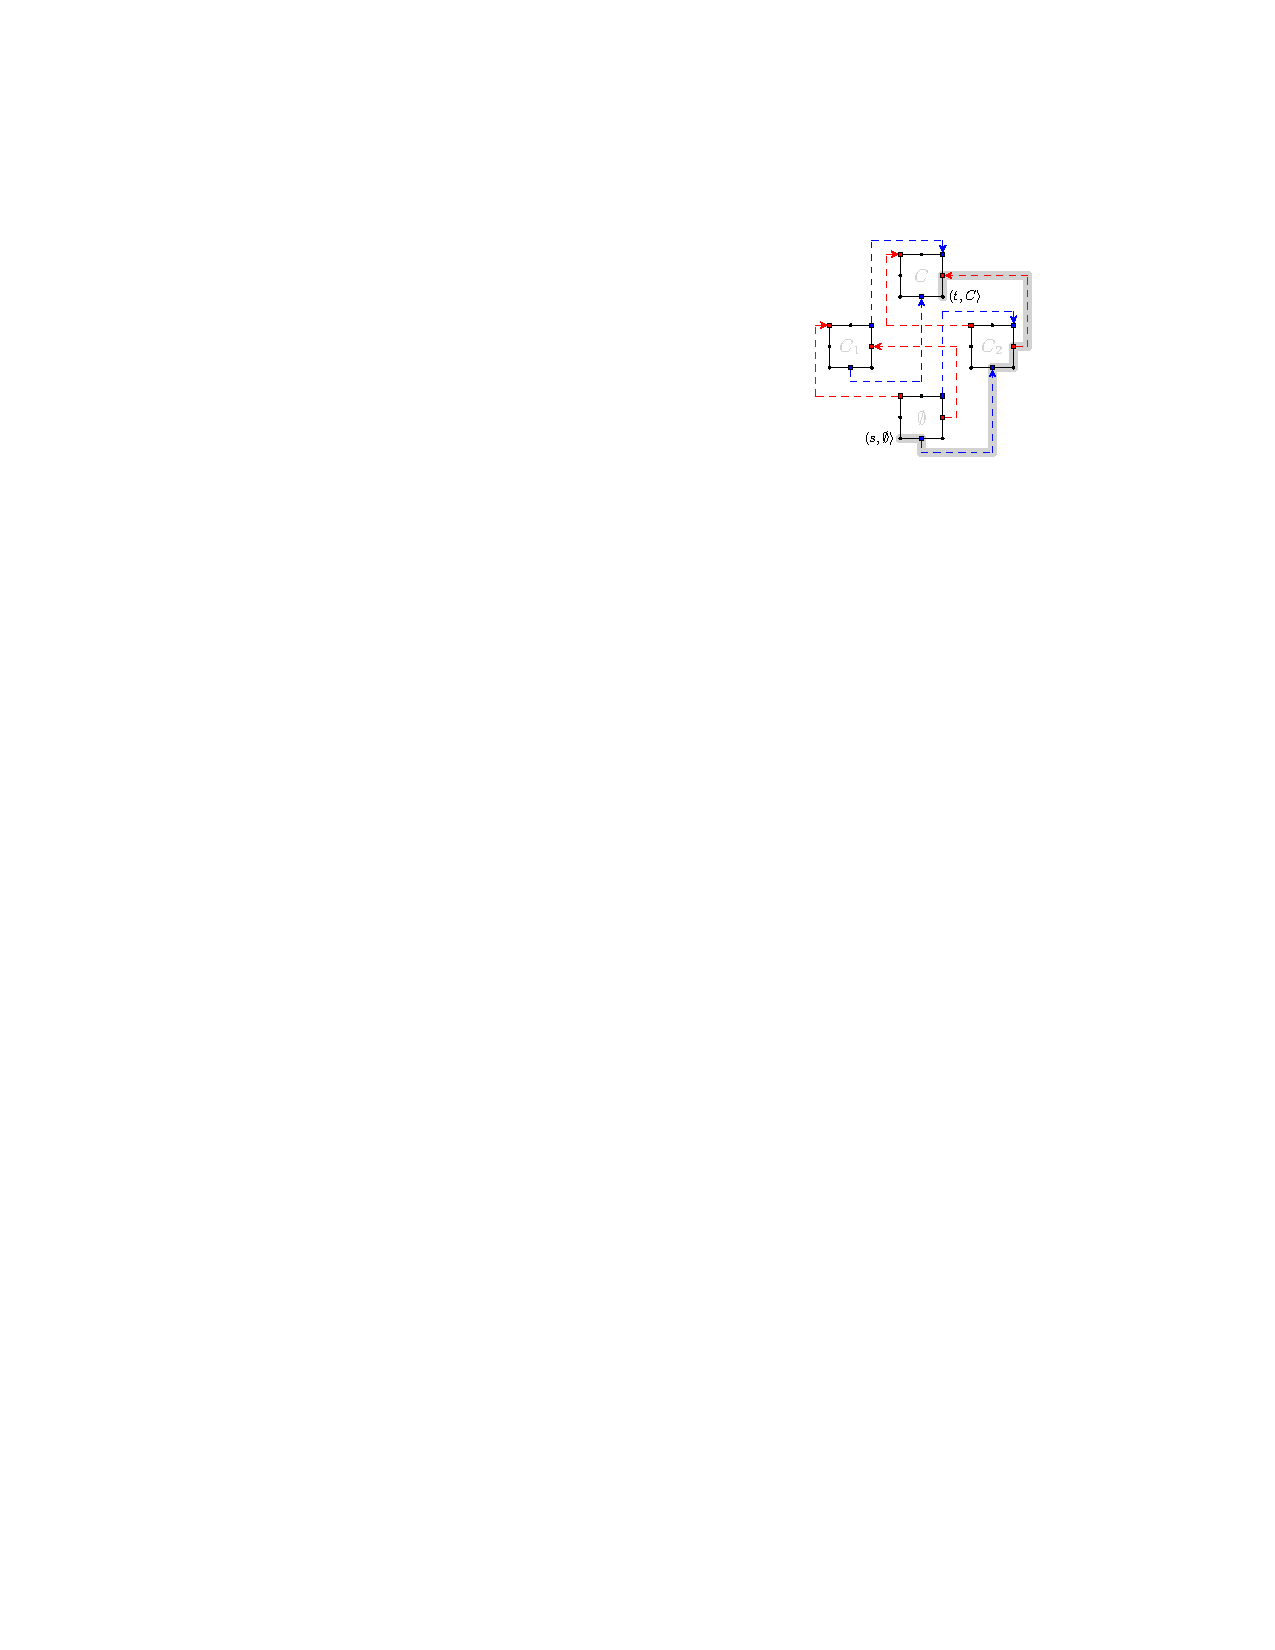
\psfig{file=ProductGraph.pdf,width=2in}
\caption{The product graph $G_{C}$ with the shortest path highlighted (taken from \cite{Rice:2013})}
\label{fig:productgraph}
\end{figure}

\subsection{The Product Graph}
\label{subs:productgraph}
The algorithm starts by constructing a \textit{product graph}. 
For a set $C$ of node subsets, the product graph is defined as $G_{C}=(V \times \mathcal{P}(C), E_{1} \cup E_{2})$, where $\mathcal{P}(C)$ is the \textit{power set}, or set of all subsets, of $C$. $E_{1}$ is the set of edges in $G$ copied for each subset of $C$, and $E_{2}$ is a set of edges from each node in each proper subset $c$ of $C$ to the same node in every other subset $c'$ such that $c$ is a proper subset of $c'$ but there are no proper subsets $c''$ of $c'$ such that $c$ is a proper subset of $c''$. This is shown in Figure~\ref{fig:productgraph}. The original graph $G$ is duplicated for every subset of $C$. The $E_{1}$ edges are within each duplicate and shown as solid lines. The $E_{2}$ edges go between the duplicates of $G$, and are shown as dashed lines. 

This construction turns the problem into a shortest-path type problem from s in the first state, the empty set, to t in the last state, C. Reaching a node from a node subset results in advancing to a state that reflects having already visited that subset. 

\subsection{Contraction Hierarchies}
\label{subs:CH}
The algorithm uses a technique known as contraction hierarchies (CH) on the product graph. This process assigns a unique rank, $\phi(u)$, to each node $u$. The method of ranking nodes used in this algorithm is from Geisberger et al. \cite{geisberger:2008}. It assigns higher values to nodes in more shortest paths. 

After the nodes are ranked, for every unique shortest path from $v$ to $w$ containing $u$, if $\phi(u)$  is less than $\phi(v)$ and $\phi(w)$, a short-cut edge is added with a cost equal to the sum of the costs of $(u,v)$ and $(v,w)$. The ``upward" graph, $G^{\uparrow}$, is defined as $(V,E^{\uparrow})$, where $E^{\uparrow}$ contains all edges $(u,v)$ such that $\phi(u) < \phi(v)$, and the ``downward" graph, $G^{\downarrow}$, is defined as $(V,E^{\downarrow})$, where $E^{\downarrow}$ contains all edges $(u,v)$ such that $\phi(u) > \phi(v)$. 

%A more detailed treatment of this step can be found in \cite{Rice:2013}.
%\subsection{Additional Preprocessing}
%\label{subs:preprocessing}


\subsection{Establishing the Upper Bound}
\label{subs:upperbd}
The next step in the algorithm is to calculate an upper bound, $\mu$, on the possible solution. This is accomplished by constructing a path on the CH product graph starting with $s$ and going along the shortest (or minimum cost) edge such that the destination node is in a node subset where no node has been visited, until all subsets have been visited. After all subsets have been visited, the total cost of the path plus the distance from the last node to $t$ is an upper bound $\mu$ on the possible cost (meaning that the optimal solution cannot have a higher cost). This is a variation of an approximate algorithm for the TSP known as the ``nearest neighbor" algorithm. 

\subsection{$\Delta$-Corridors}
\label{subs:deltacorridors}

The next step in the algorithm is to establish $\Delta$-corridors. $\Delta$-corridors are based on the idea that it's not necessary to consider nodes that are far away from the space between $s$ and $t$, assuming that there are nodes from all node subsets near the direct path between $s$ and $t$. 

This step establishes $V_{\Delta}$, defined as $V_{\Delta}=\{v \in V | d(s,v) + d(v,t) \leq \Delta \}$. To find this, Dijkstra's algorithm, a shortest-path algorithm, is used on the CH graph once from $s$ on $G^{\uparrow}$ and once from $t$ on $G^{\downarrow}$. The details of this step can be found in \cite{Rice:2013}. The algorithm uses $\Delta = \mu /(1+\epsilon)$, where $\epsilon \geq 0$. If $\epsilon=0$, this algorithm is an exact algorithm. 

\subsection{A* Search}
\label{subs:A*}
In $A^{*}$ search, a value is assigned to each node with the formula $f(v)=d(v)+h(v)$, where $d(v)$ is the cost of the minimum cost known path from the starting node $s$ to $v$ and $h(v)$ is the estimated cost for minimum cost path from $v$ to the end node $t$. 

The algorithm begins by inserting all nodes adjacent to $s$ into a set $F$, the ``fringe" set, and setting $d(s)=0$. For all other nodes, $d(v)$ is defined as $\infty$.

Next, a node $u$ with minimum $f$ value (as defined above) is removed from $F$. For every node $v$ adjacent to $u$, if $d(v) > d(u) + c(e)$, where $e$ is the edge between $u$ and $v$, then $d(v)$ is set to be $d(u) + c(e)$ and $v$ is inserted into $F$. This is repeated until $t$ is reached and chosen to be removed from $F$, when $d(t)$ is returned. 

The algorithm uses $A^{*}$ search on the CH product graph within $V_{\mu / (1+\epsilon)}$, the $\Delta$-corridor established in Section~\ref{subs:deltacorridors}. Rice and Tsotras \cite{Rice:2013} prove that their $A^{*}$ search heuristics will return the correct shortest path. 

After $A^{*}$ search is completed, $min\{\mu,w(P^{*})\}$ is returned, where $\mu$ is the upper bound calculated in Section~\ref{subs:upperbd} and $P^{*}$ is the path calculated in $A^{*}$ search. Rice and Tsotras \cite{Rice:2013} prove that this algorithm runs in $O^{*}(2^{k})$ time, where $k$ is the number of node subsets and the $O^{*}$ notation means that polynomial factors are omitted. 

\subsection{Experimental Results}
\label{subs:riceresults}
Rice and Tsotras \cite{Rice:2013} conducted experiments using the road network of North America. 

In the first experiment, the algorithm was implemented with the number of subsets $V_{i}$ fixed at 5, varying $\epsilon$ and the numbers of nodes in each subset. They found that query time decreased from 1 second to 0.002 seconds as the numbers of nodes increased from $10$ to 1,000,000. The query time also decreased as $\epsilon$ increased. The cost of the solutions found are worse than optimal by less than 25\%, and are significantly lower in most cases. 

In the second experiment, the number of nodes in each subset was fixed at 10,000 and the number of nodes and $\epsilon$ were varied. The results showed errors of less than 5\%.

\section{Local-Global Search and Consultant Guided Search}
\label{sec:genetic}
Often, combining several algorithms to make a hybrid algorithm can generate an algorithm that is more effective than the original algorithms alone. This can be useful for solving NP-hard optimization problems like the GTSP. 
In this section, I present an algorithm from Pop and Iordache \cite{Pop:2011}. This algorithm is a hybrid of two algorithms: local-global search and consultant-guided search (CGS). Unlike the algorithm in Section~\ref{sec:parameterized}, this algorithm assumes that the nodes in each node subset are close together. 

\subsection{Local-Global Search}
\label{subs:localglobal}

\begin{figure}
\centering
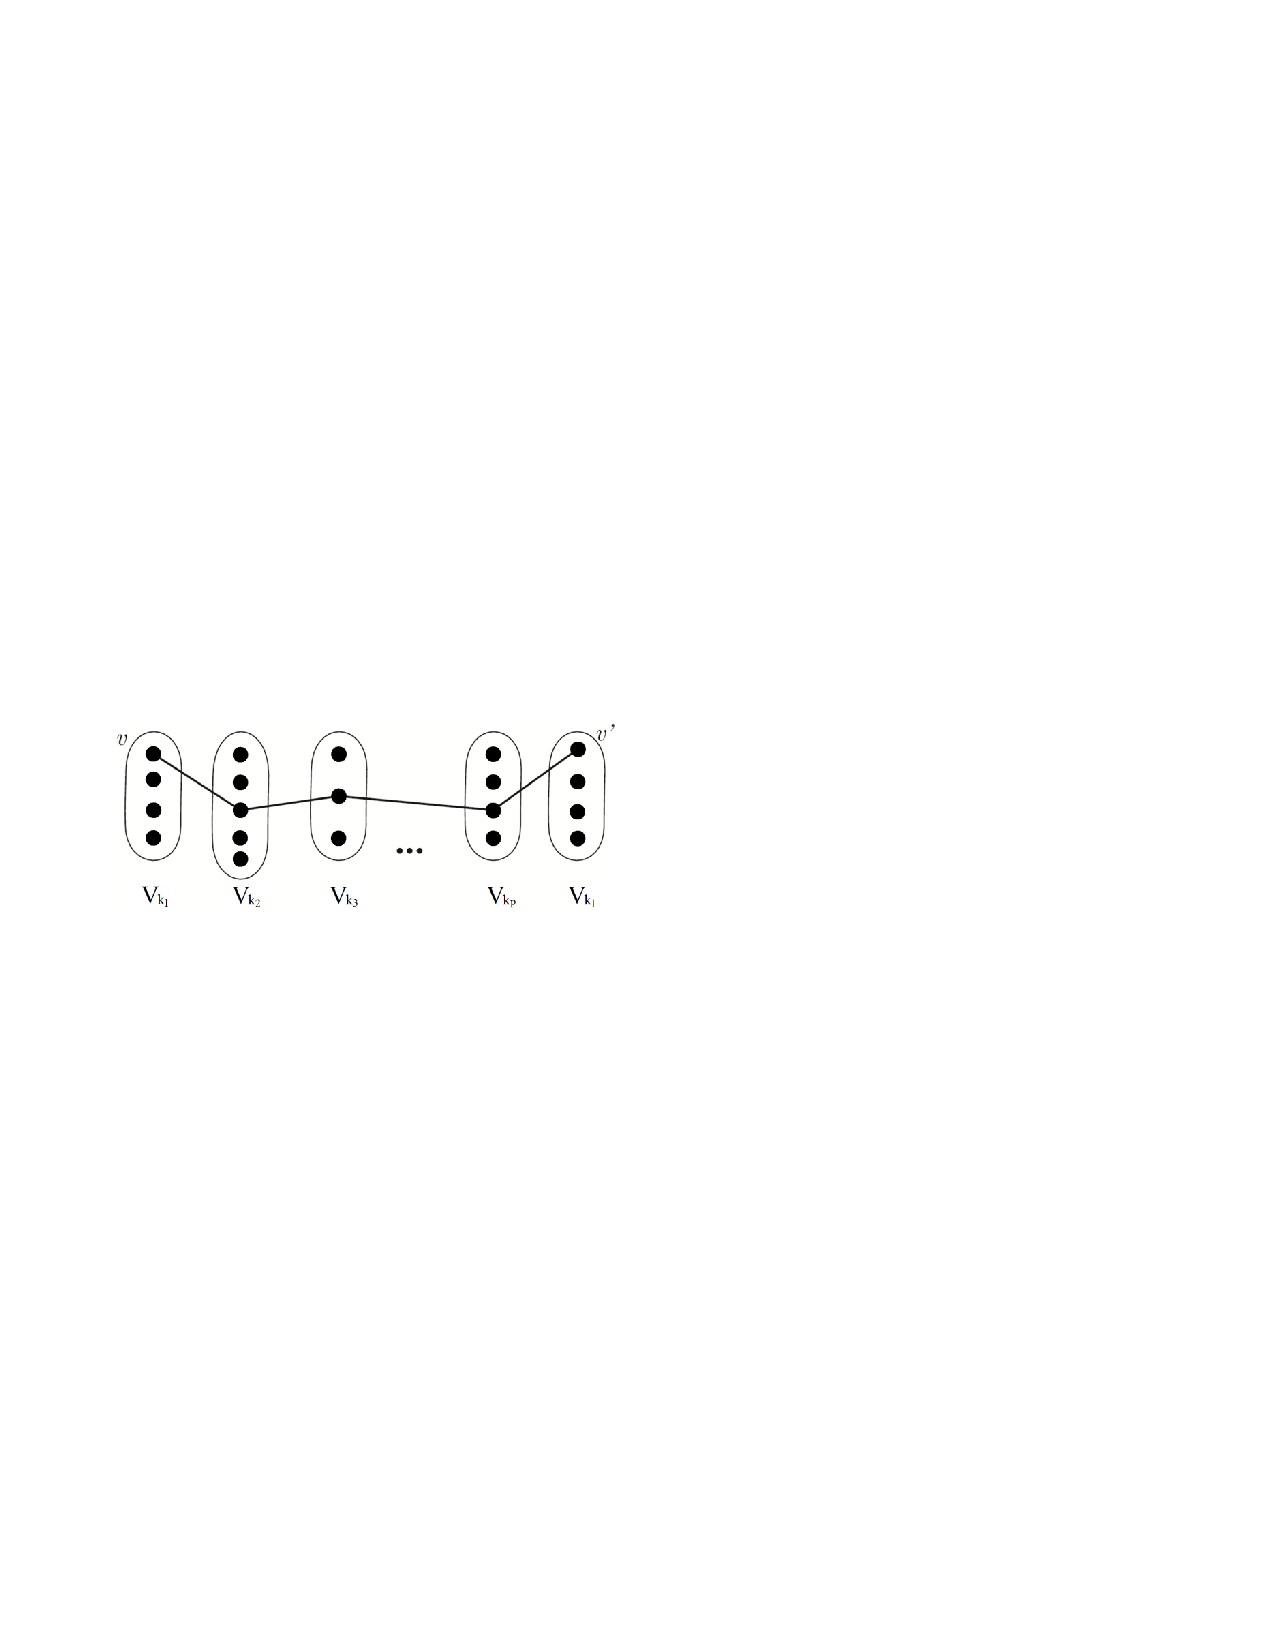
\psfig{file=PopImage1.pdf,width=3in}
\caption{The local-global approach (taken from \cite{Pop:2011})}
\label{fig:localglobal1}
\end{figure}
Local-global search is a technique that distinguishes between edges connecting nodes within the same subset and edges connecting nodes of different subsets. 

A new graph, $G'$, is constructed with a supernode that represents each subset $V_{i}$. Supernodes are denoted with the name of the subset $V_{i}$.

Given a sequence of supernodes $V_{k_{1}},V_{k_{2}},...,V_{k_{n}}$, the local-global search algorithm finds the minimum-cost cycle that visits one node from each subset in the order of the sequence. This is accomplished by duplicating $V_{k_{1}}$ and putting it at the end of the sequence, then considering each path from each node in $V_{k_{1}}$ to the corresponding node in $V_{k_{n+1}}$, visiting the subsets in the order of the sequence, as shown in Figure~\ref{fig:localglobal1}.

\begin{figure}
\centering
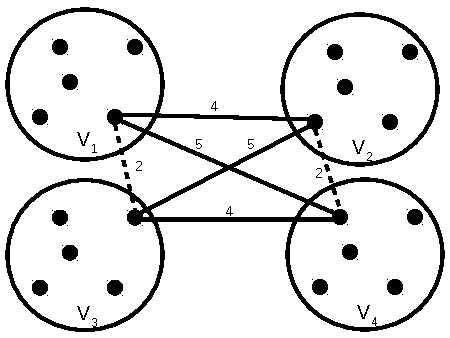
\psfig{file=localglobal2revised.pdf,width=3in}
\caption{Local-global search given the sequence $(V_{1},V_{2},V_{3},V_{4})$, with costs as labeled}
\label{fig:localglobal2}
\end{figure}

This algorithm is a polynomial time algorithm. This may seem like it contradicts the GTSP being an NP-hard problem. However, the algorithm does not actually find the overall optimal solution for the GTSP; rather, it only finds the optimal solution for a particular sequence of node subsets. One example of this is shown in Figure~\ref{fig:localglobal2}. This is indeed the shortest cycle given the sequence $(V_{1},V_{2},V_{3},V_{4})$, but it's not the best solution overall. An optimal solution would use the same nodes with the dotted edges and the sequence $(V_{1},V_{2},V_{4},V_{3})$, but local-global search doesn't rearrange the sequence order. Using the algorithm to find the optimal solution over all possible sequences is an exponential time algorithm, as expected. 

\subsection{Consultant-Guided Search}
\label{subs:CGS}
Consultant-guided search is also used. The following information is from Iordache  \cite{Iordache:2010}. 

Consultant-guided search (CGS) is a swarm intelligence algorithm, meaning that it is decentralized. It is based on the way people take advice from consultants. 

The algorithm has simulated individuals that take on two roles, consultants and clients. Each iteration, each virtual client chooses a virtual consultant based on the consultants' \textit{reputation}. A consultant's reputation increases when the consultant's clients succeed. A \textit{success} is defined as a solution that is better than any other solution that has been found by the algorithm. Reputation generally decreases over time unless prevented by successes. The exception to this rule is that for some consultants who have had a very high reputation at some point, the reputation is prevented from going below a certain level. 

Another factor that influences a client's choice is the consultant's \textit{personal preference}. This factor is different for each problem where CGS is used. 

In addition to reputation, each consultant also has a \textit{strategy}, which they use to help the client to solve the problem. Using the strategy, the consultant offers a suggestion, and the client may or may not take the suggestion offered. This introduces some randomness into the construction process. 

The consultants also have a \textit{sabbatical} mode, where they do not give advice to clients and change their strategy. Sabbatical mode is activated if the consultant's reputation goes below a certain level, and is deactivated after a certain amount of time. 

\subsection{The Hybrid Algorithm}
\label{subs:pophybrid}
The algorithm Pop and Iordache propose is a hybrid of the local-global and CGS techniques. 

The consultant uses virtual distances between subsets as described in Section~\ref{subs:localglobal}, with each supernode at the center of mass of the subset, to generate a cycle that visits all supernodes. This cycle is improved with methods that are beyond the scope of this paper, and can be found at \cite{Pop:2011}. The consultant then uses this cycle to advise the clients. In each step of generating the cycle, the consultant randomly chooses the next supernode from the supernodes not yet visited within a candidate list of the $n$ closest supernodes. The probability of choosing supernode $j$ from supernode $i$ is given by the formula 
\begin{align*}
p^{k}_{ij}=\frac{1/d_{ij}}{\sum_{l \in \mathcal{N}^{k}_{i}}(1/d_{il})}
\end{align*} 
where $\mathcal{N}^{k}_{i}$ is the set of possible supernodes and $d_{ij}$ is the distance between the two supernodes $i$ and $j$. 

When a client chooses a consultant, the consultant recommends the next subset for the client to visit. The consultant accomplishes this by looking at the client's current supernode and finding it in the consultant's constructed cycle. If the client has not visited either the supernode before or after the client's current supernode, the consultant will recommend the one that has not yet been visited, or randomly pick one of the two if neither one has been visited. If the client has already visited both supernodes, the consultant does not make a recommendation. 

The client may or may not take this recommendation. If there are still supernodes within the candidate list that have not been visited by the client, the client's choice is dictated by the formula
\begin{align*}
j = \left\{
        \begin{array}{ll}
            v & \quad v \neq \textrm{null} \wedge q \leq q_{0} \\
            \textrm{random}\left(\mathcal{N}^{k}_{i}\right) & \quad \textrm{otherwise}
        \end{array}
    \right.
\end{align*}

where $i$ is the current node subset, $v$ is the recommended node subset, $q_{0}$ is a parameter, and $q$ is a random variable between 0 and 1 (inclusive). 

If all supernodes in the candidate list have been visited, the client chooses a supernode not in the candidate list.

After a sequence of supernodes is chosen, the local-global search technique in Section~\ref{subs:localglobal} is used to find the best overall cycle. 

\subsection{A variant using confidence}
Pop and Iordache also present a variant where each consultant's confidence in each edge of a cycle factors in the client's decision to take the suggestion. In this variant, each edge in a consultant's strategy cycle has a strength. When a consultant uses an edge in the cycle for the first time, it is given a strength of 0. Each time the consultant re-uses the same edge, the edge's strength is incremented. A client is more likely to choose the recommended supernode if the edge between the supernodes has a higher strength. 

\subsection{Experimental Results}
\label{subs:popresults}
The algorithm and the variant with confidence were tested on GTSP instances adapted from TSP instances from the TSPLIB library \cite{Reinelt:1991}. The results from the algorithm variant with confidence were statistically similar to the best known heuristic at the time the paper was written, and in some cases, the variant with confidence was significantly better. 

\section{Variable Neighborhood Search}
\label{sec:VNS}
This section presents another algorithm that combines several techniques, this time using variable neighborhood search. Although this algorithm was originally presented by Hu and Raidl \cite{Hu:2008}, most of what is presented below is from Pourhassan and Neumann \cite{Pourhassan:2015}. Pourhassan and Neumann present some instances that illustrate the strengths and weaknesses of each individual technique and the combined algorithm. 

\subsection{Cluster-Based Local Search}
\label{subs:CBLS}
The cluster-based approach starts with a permutation of the node subsets (or \textit{clusters}), then finds the optimal set of nodes within the clusters for this permutation. First, a permutation of clusters $\pi = (V_{k_{1}}, V_{k_{2}}, ..., V_{k_{m}})$ is chosen. The \textit{2-opt neighborhood} of $\pi$ is defined as 
%\begin{flalign*}
%&N(\pi) = \left\{\pi' | 1 \leq i < j \leq m, \right.
%\\
%&\left.\pi' = (\pi_{1},...,\pi_{i-1},\pi_{j},\pi_{j-1},...,\pi_{i},\pi_{j+1},...,\pi_{m})\right\}
%\end{flalign*}
\begin{flalign*}
&N(\pi) = \left\{\pi' | 1 \leq i < j \leq m, \right.
\\
&\left.\pi' = (V_{k_{1}},...,V_{k_{i-1}},V_{k_{j}},V_{k_{j-1}},...,V_{k_{i}},V_{k_{j+1}},...,V_{k_{m}})\right\}
\end{flalign*}
where $m$ is the number of clusters. In other words, part of $\pi$ is reversed (specifically, the part between $V_{k_{i}}$ and $V_{k_{j}}$). Note that this does not include all possible permutations of the node subsets. 

Cluster-based local search (CBLS) searches through every permutation from the 2-opt neighborhood of $\pi$ and finds optimal nodes for the permutation. For each permutation, if the cost of the cycle is less than the cost of the current lowest cost cycle, that cycle is stored as the new lowest cost cycle and $\pi$ is set to the new permutation. This finds the minimum cost cycle from the permutations that are tried. 

\subsection{Node-Based Local Search}
\label{subs:NBLS}
The node-based approach starts with a set $P$ of one node from each cluster, then finds the minimum-cost cycle within that set. Note that the second step is basically the standard TSP, as described in Section~\ref{subs:GTSP}. Because the TSP is NP-hard, this step cannot be solved optimally in polynomial time, although this doesn't matter much if the number of clusters is small. Alternatively, an approximate algorithm for the TSP may be used here. Pourhassan and Neumann \cite{Pourhassan:2015} present two algorithms used in this step--one that finds an optimal solution and one that approximates a solution.

The neighborhood of the set $P$ of nodes can be described formally as

\begin{align*}
N'(P) = \left\{P' | P' = \{p_{1},...,p_{i-1},p'_{i},p_{i+1},...,p_{m}\},\right.
\\
\left. p'_{i} \in V_{i} \backslash \{p_{i}\},1 \leq i \leq m \right\}
\end{align*}

In other words, the neighborhood of $P$ is given by all possible sets $P'$ where one node $p_{i}$ is removed from $P$ and a different node in the same subset as $p_{i}$ is added. 

The algorithm first finds the solution for $P$, then searches the neighborhood of $P'$. If the solution found for $P'$ is better than the current best solution, the new solution is set as the current best and $P'$ is set as $P$. The algorithm terminates when there are no better solutions found for the neighborhood of $P$. 

\subsection{Variable Neighborhood Search}
\label{subs:VNS}
The Variable Neighborhood Search algorithm combines cluster-based local search and node-based local search into one algorithm. The combined algorithm starts with a possible solution $(P,\pi)$, where $P$ is a set of nodes and $\pi$ is a permutation of clusters, then uses two neighborhood types based on the two algorithms, which can be defined as
\begin{itemize}
\item $N_{1}(P) = \left\{(P',\pi') | \pi' \in N(\pi), P'= \right.$ optimal set of nodes with respect to $\left. \pi' \},\right.$
\item $N_{2}(\pi) = \left\{(p',\pi') | P' \in N'(P),\pi'=\right.$ order of clusters obtained by 2-opt from $\pi$ on $\left. G[P']\right\}$
\end{itemize}

First, $N_{1}$ is used along with the CBLS algorithm to find a possible solution. When this is found, $N_{2}$ is used with NBLS, using $P$ and $\pi$ as found by $N_{1}$. 

\subsection{Example Instances}
\label{subs:instances}
Approximate algorithms usually have some cases that are easier for them than others. This section presents some of these cases. 

\begin{figure}[t]
\centering
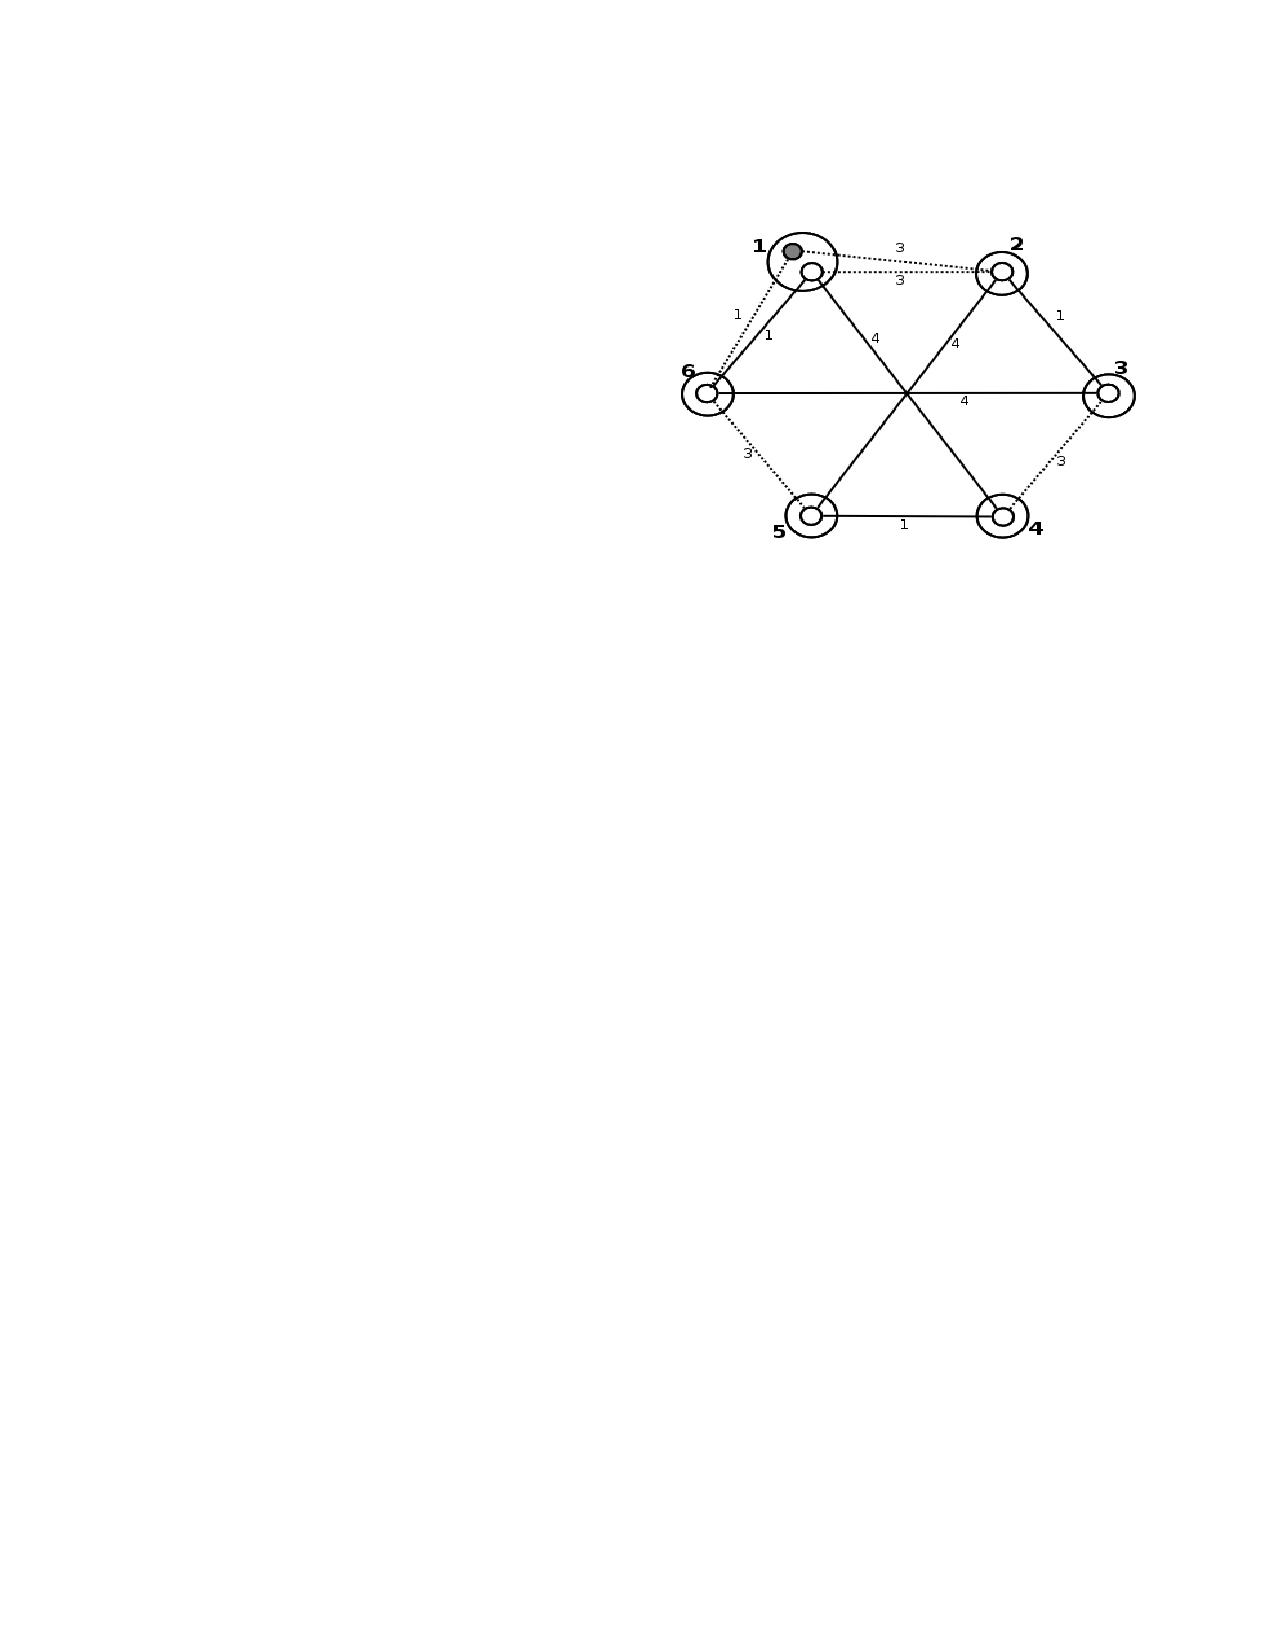
\psfig{file=GTSPCase1.pdf,width=3in}
\caption{The first instance (taken from \cite{Pourhassan:2015})}
\label{fig:Pourhassan1}
\end{figure}

The first instance is one that is difficult for the cluster-based local search technique, but easy for the node-based local search technique. The graph for this instance is shown in Figure~\ref{fig:Pourhassan1}. The optimal solution would visit the nodes using the edges on the sides of the graph, and not use the edges with cost 4. However, Pourhassan and Neumann \cite{Pourhassan:2015} prove that if the starting permutation is $\pi=(1,4,5,2,3,6)$, then the cluster-based local search algorithm will never find one of these solutions, but node-based local search does. 

\begin{figure}[h]
\centering
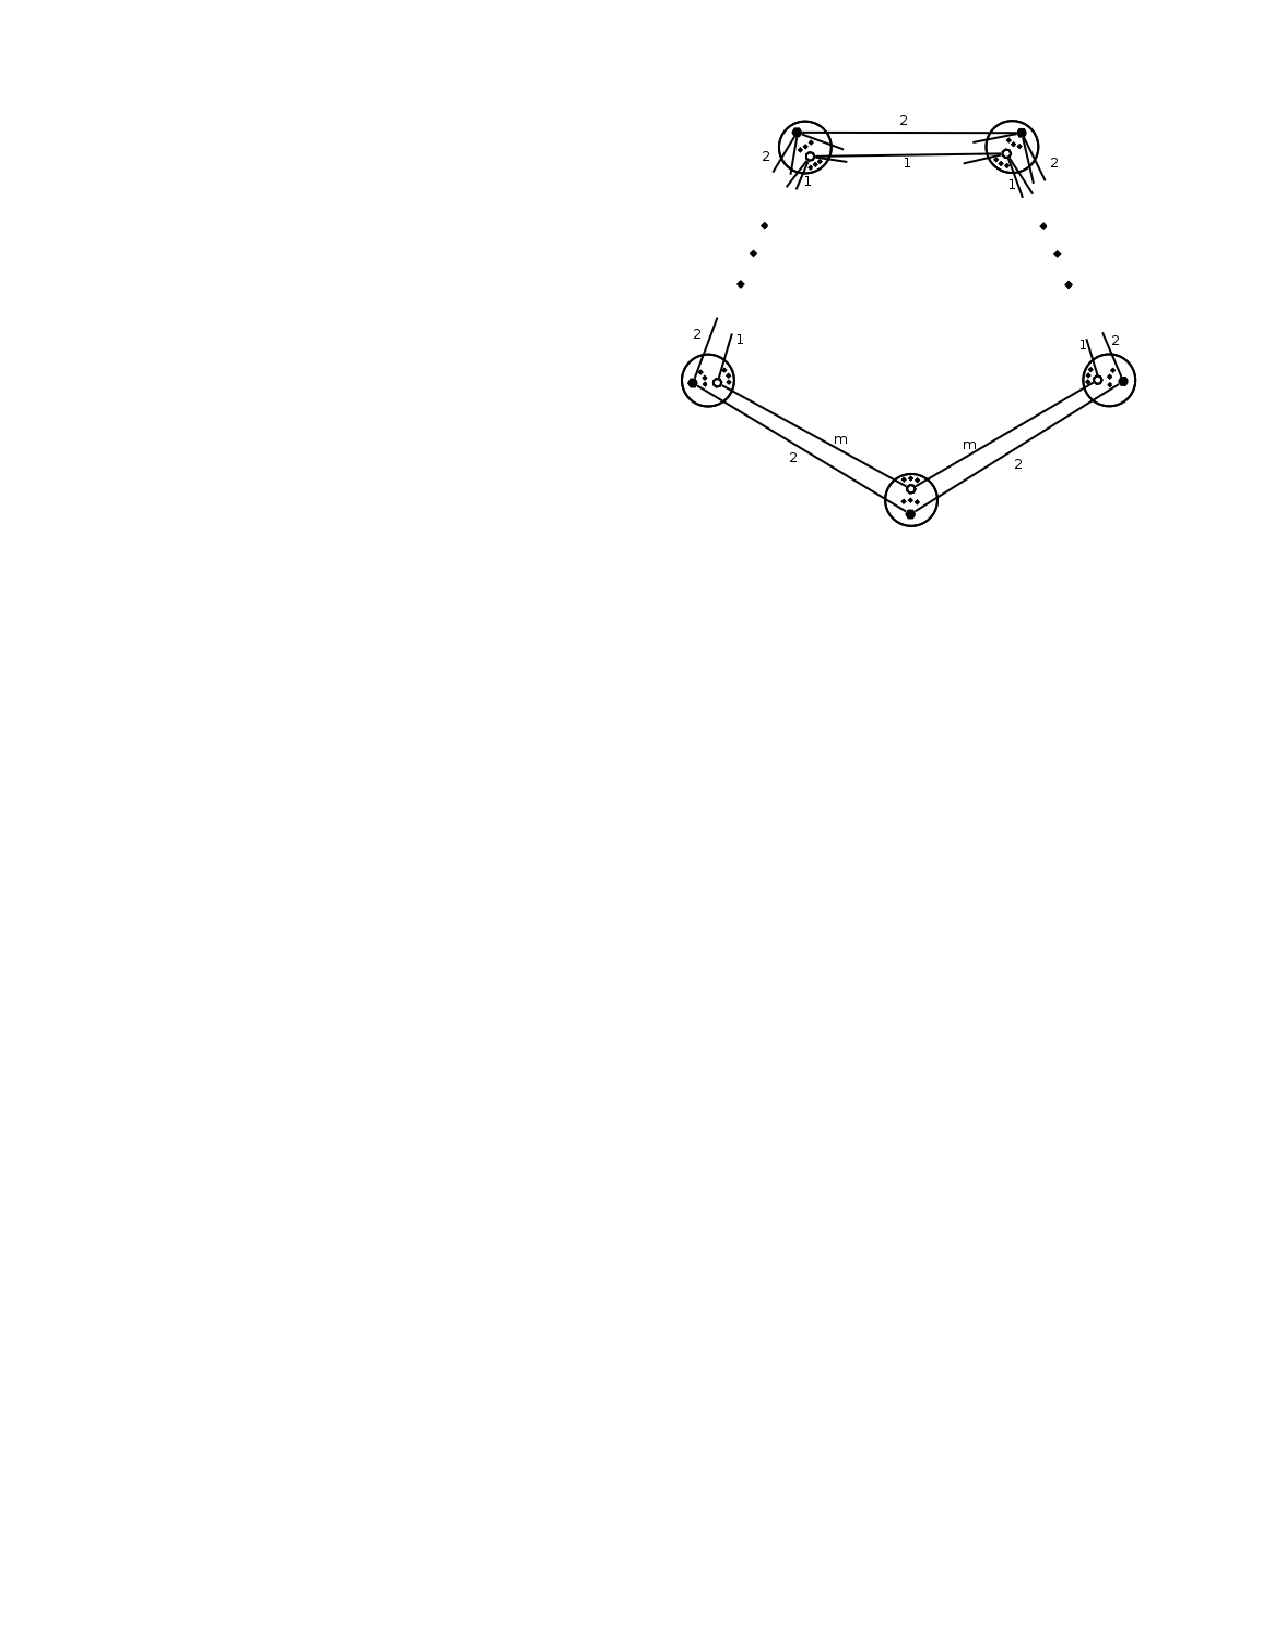
\psfig{file=GTSPCase2.pdf,width=3in}
\caption{The second instance (taken from \cite{Pourhassan:2015})}
\label{fig:Pourhassan2}
\end{figure}

The second instance is difficult for node-based local search, but easy for cluster-based local search. This instance is shown in Figure~\ref{fig:Pourhassan2}. The instance includes one cluster with a black node that is closer to the other clusters and a white node that is farther away. The optimal solution uses all black nodes. Pourhassan and Neumann \cite{Pourhassan:2015} prove that cluster-based local search is able to find an optimal solution, whereas node-based local search gets stuck in local optima. 

\begin{figure}
\centering
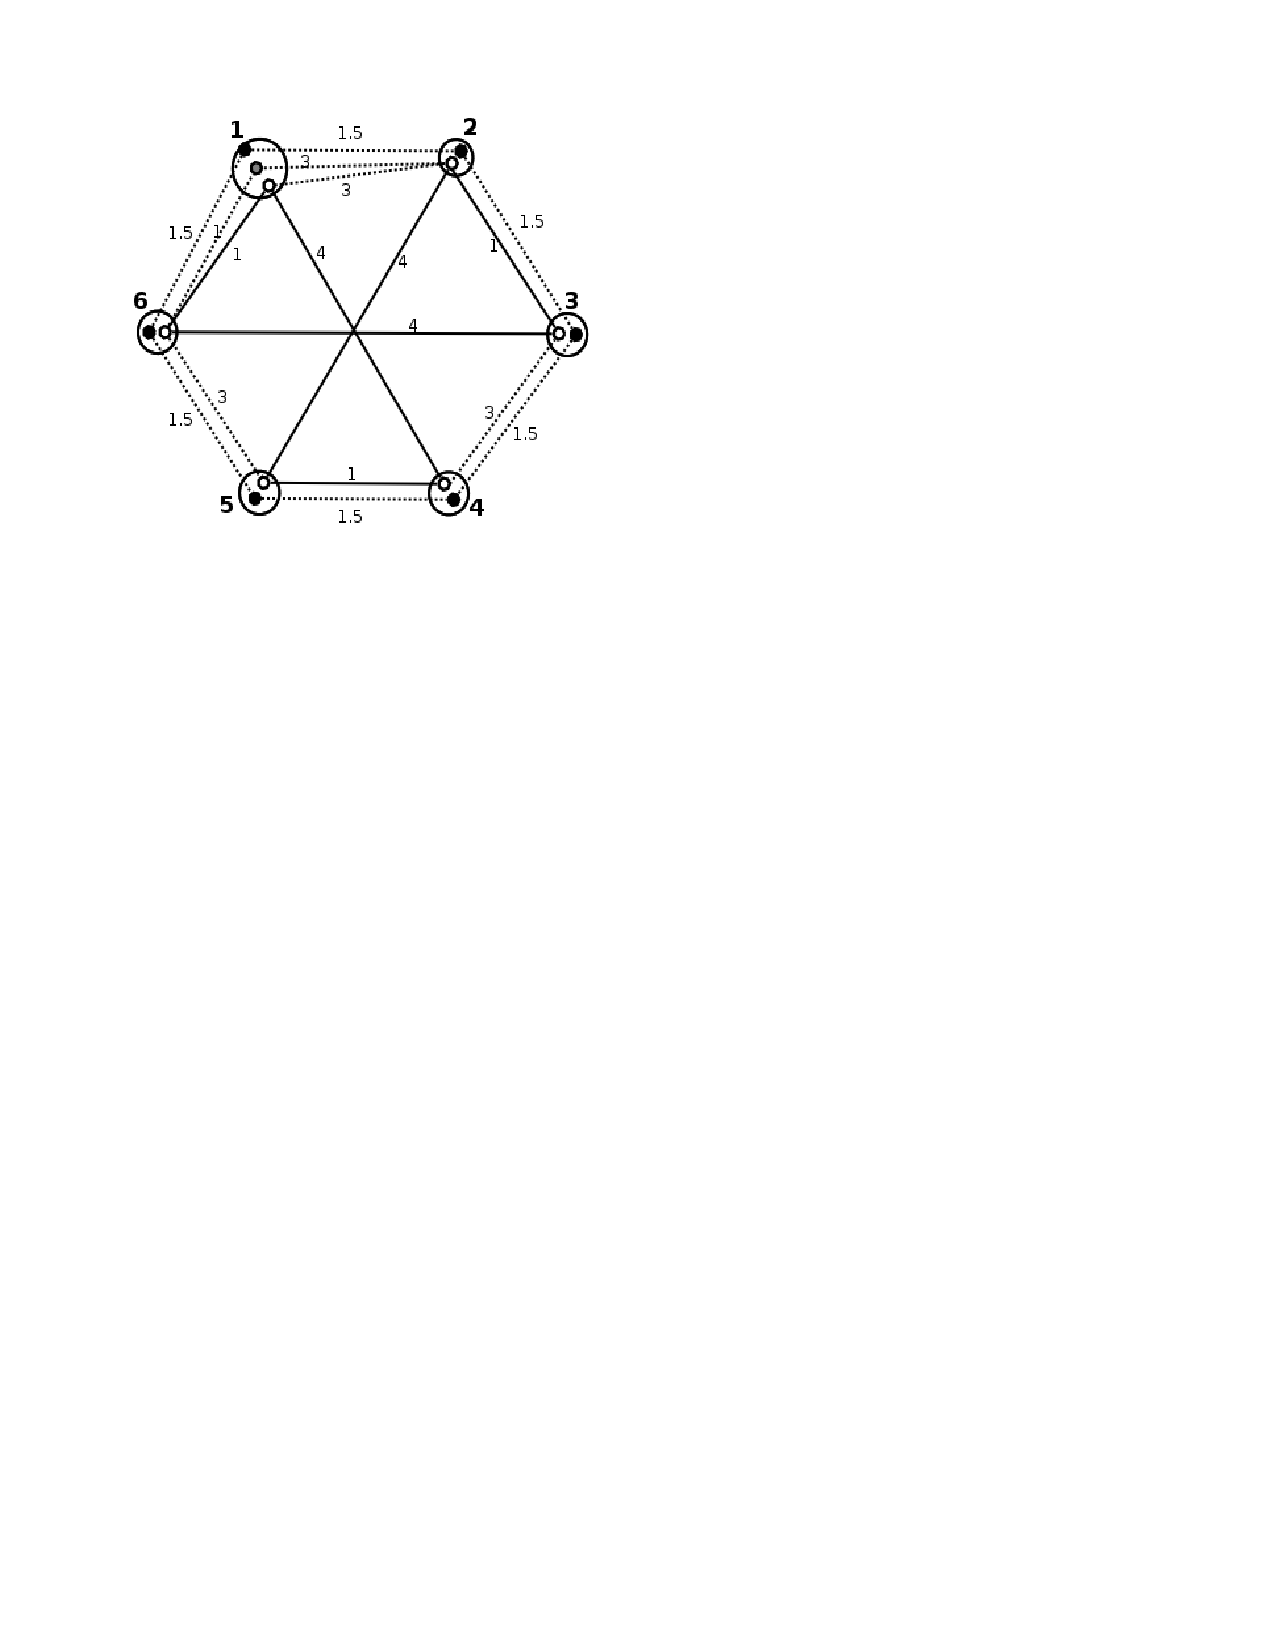
\psfig{file=GTSPCase3.pdf,width=3in}
\caption{The third instance (taken from \cite{Pourhassan:2015})}
\label{fig:Pourhassan3}
\end{figure}

The third instance is shown in Figure~\ref{fig:Pourhassan3}. This instance combines the first two, with the basic structure of the first one, but with varying lengths of edges between nodes of the same clusters. This makes the instance hard for both cluster-based and node-based local search. Variable-neighborhood search, however, doesn't get stuck and can find a good approximation. This illustrates the advantages of variable-neighborhood search. 

\section{Conclusions}
\label{sec:conclusions}
I have summarized three heuristics for the GTSP. Although the GTSP is NP-hard and exact algorithms are often time-consuming, approximate algorithms are effective for many practical purposes. Additionally, as Rice and Tsotras \cite{Rice:2013} show, there are specific cases where in practice, exact algorithms are feasible. 

There are many different applications of the GTSP, and sometimes, the application changes which algorithm would work best. Rice and Tsotras \cite{Rice:2013} apply their algorithm for road trips, which assumes that elements of each node subset are spread out. Pop and Iordache \cite{Pop:2011} mention that they assume the nodes in each subset are near each other. As Pourhassan and Neumann \cite {Pourhassan:2015} point out, factors like the distance between node subsets and nodes in subsets make a significant difference in how well an algorithm will work. A good heuristic should produce good approximations in a variety of cases, but when choosing a heuristic, it's important to consider the application. 

\section{Acknowledgements}
I would like to thank Elena Machkasova, Nic McPhee, and Max Magnuson for their feedback on this paper. I would also like to thank Michael Rice and Vassilis Tsotras for answering questions about their work and providing a copy of one of their earlier papers. 

%\subsection{References I haven't cited yet}
%\cite{Pop:2011}, \cite{Pourhassan:2015}, \cite{Hu:2008}
%\todo[inline, color=light-gray]{This subsection only exists so my references will show up. I will delete it after I cite them elsewhere in the paper.}
% The following two commands are all you need in the
% initial runs of your .tex file to
% produce the bibliography for the citations in your paper.
\bibliographystyle{abbrv}
% sample_paper.bib is the name of the BibTex file containing the
% bibliography entries. Note that you *don't* include the .bib ending here.
\bibliography{sample_paper}  
% You must have a proper ".bib" file
%  and remember to run:
% latex bibtex latex latex
% to resolve all references

\end{document}
